Para la lectura del fichero almacenado en la memoria FLASH del dispositivo, el cual contiene las medidas obtenidas por los sensores,se ha desarrollado un programa independiente el cual se encarga de realizar esta función. Además, permite la eliminación de dicho fichero. Para ejecutar dichas funciones, se enviará por serial al micro un caracter u otro mediante el teclado. Ambas operaciones de realizan mediante el sistema de archivos SPIFFS.


Para la realización de este programa, se ha utilizado las funciones \texttt{Clear\_file} y \texttt{Read\_meas} explicadas en el \autoref{subsubsec:ManejadorFicheros}, por lo que ha sido necesario importar el archivo \texttt{file\_management.hpp}, el cual contiene las definiciones de dichas funciones.

Este programa se puede divir en dos partes, la función \texttt{setup()}, la cual se ejecuta tan solo una vez al arracar el programa, y la función \texttt{loop()}, la cual consiste en un bucle infinito con el principal funcionamiento del programa. A continuación, se va a explicar el funcionamiento de estas dos funciones:

\begin{itemize}
    \item \texttt{setup()}: esta función tan solo inicializa el serial a una velocidad de 9600 bps, y muestra el siguiente mensaje por serial al usuario:
    \begin{figure}[H]
        \centering
        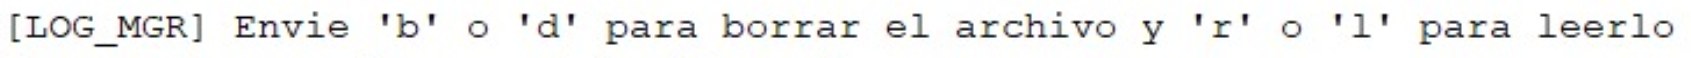
\includegraphics[width=0.8\textwidth]{images/3-software/3-4-readfile/MensajeInicial.png}
        \caption{Mensaje inicial programa de lectura}
        \label{fig:3-4-1-MensajeInicial}
    \end{figure}
    \item \texttt{loop()}: contiene el principal funcionamiento del programa y su secuencia de ejecución es la seguiente:
    \begin{enumerate}
        \item Verificar si el serial funciona correctamente. En caso de que el serial no esté en pleno funcionamiento, el programa no hace nada.
        \item Lee el caracter enviado mediante el serial y lo guarda en una variable.
        \item En caso de que dicho caracter sea una 'b' o una 'd', se procede a la secuencia de eliminación del fichero. Dicha secuencia es la siguiente:
        \begin{enumerate}
            \item Se muestra por serial un mensaje indicando al usuario la acción realizada.
            \item Se llama a la función \texttt{clear\_file}, incluida en la librería \texttt{file\_management.hpp}, pasandole como parámetro el archivo a eliminar.
            \item Una vez eliminado el fichero, se realiza una comprobación de la existencia de dicho archivo, mostrando por serial el estado del archivo.
            \item Se cierra el archivo.
        \end{enumerate}
        \item Por otra parte, en caso de que el caracter leído haya sido una 'r' o una 'l', se procede a la lectura del fichero, llamando a la función \texttt{read\_meas}, en la librería \texttt{file\_management.hpp}, pasandole como parámetro el archivo a leer.
        \item En caso de que el caracter no haya sido ninguno de los anteriores mencionados, el sistema muestrará por serial el mismo mensaje que al principio de la ejecución de este programa, indicando al usuario que caracteres son aceptados.
    \end{enumerate}
    \begin{lstlisting}[captionpos=b, caption={Programa lectura o eliminación de fichero}, language=c++]
        #include "file_management.hpp"

        const char* testFile = "/measurements.txt";

        void setup() {
          Serial.begin(9600);
          Serial.println("[LOG_MGR] Envie 'b' o 'd' para borrar el archivo y 'r' o 'l' para leerlo ");
        }

        void loop() {
            // Verificar si hay datos disponibles en el puerto serial
            if (Serial.available() > 0) {
                char command = Serial.read(); // Leer el caracter ingresado
                if (command == 'b' ||  command == 'd') {

                    Serial.println("[LOG_MGR]Borrando contenido del archivo...");
                    clear_file(testFile);

                    // Confirmar estado del archivo despues de borrarlo
                    File file = SPIFFS.open(testFile, "r");
                    if (file && file.available()) {
                        Serial.println("[LOG_MGR] El archivo aun tiene contenido.");
                    } else {
                        Serial.println("[LOG_MGR] El archivo esta vacio.");
                    }
                    file.close();
                } else if (command == 'r' ||  command == 'l') {
                    read_meas(testFile);
                } else if (command != '\n') {
                  Serial.println("[LOG_MGR] Envie 'b' o 'd' para borrar el archivo y 'r' o 'l' para leerlo ");
                }
            }
        }
    \end{lstlisting}
\end{itemize}

